\documentclass[pagesize=pdftex,paper=a4,bibtotoc,12pt]{scrreprt}

%%%%%%%%%%%%%%%%%DATEN%%%%%%%%%%%%%%%%%
%Erstellungsdatum
\date{\today}
%Autor
\author{Martin Kraus, Philipp Schwarz}
\title{Seminar Topologie: Kompakte Räume}

%%%%%%%%%%%%%%%%%pakete%%%%%%%%%%%%%%%%%
%neue Rechtschreibung
\usepackage{ngerman}
 
%\usepackage[T1]{fontenc}
%Umlaute ermölichen utf8 ( latin1)
\usepackage[utf8]{inputenc}
 
% Tabellen
\usepackage{array}
 
% Schriftfarben
\usepackage{color}

%Bilder
\usepackage{float}
\usepackage{floatflt}
\usepackage[pdftex]{graphicx}
\DeclareGraphicsRule{*}{mps}{*}{}
%Math
\usepackage{amsmath}
\usepackage{amssymb}

%Nomenclature
\usepackage[intoc]{nomencl}

%Kopf-/Fußzeilen
\usepackage{fancyhdr}

%Hyperref für Bookmarks im PDF
\usepackage[pdftex, pagebackref]{hyperref}

%%%%%%%%%%%%%%%%%%%%seitencfg%%%%%%%%%%%%%%%%%%%%%%%%%%%%
\pagestyle{fancy}
\fancyhf{}
%Kopfzeile links bzw. innen
\fancyhead[L]{\nouppercase{\leftmark}}
%Kopfzeile rechts bzw. außen
\fancyhead[R]{\thepage}
%Linie open
\renewcommand{\headrulewidth}{0.5pt}
%Fußzeile links bzw. innen
\fancyfoot[L]{\copyright Seminar Topologie: Kompakte Räume - Martin Kraus, Philipp Schwarz}
%Fußzeile rechts bzw. außen
\fancyfoot[R]{\today}
%Linie unten
\renewcommand{\footrulewidth}{0.5pt}

\usepackage[pdftex, pagebackref]{hyperref}
\hypersetup {
pdftitle = {Martin Kraus, Philipp Schwarz},
pdfsubject = {Seminar Topologie: Kompakte Räume}, 
pdfauthor = {Martin Kraus, Philipp Schwarz},
pdfhighlight = {/O},
pdfkeywords = {Kompakte Räume, Satz von Heine-Borel}, colorlinks = {false},
bookmarksnumbered = {true},
citebordercolor = {1 1 1},
linkbordercolor = {1 1 1},
urlbordercolor = {1 1 1},
bookmarksopen = {true},
bookmarksopenlevel = {1}
}
%%%%%%%%%%%%%%%%%%%EIGENE-BEFEHLE%%%%%%%%%%%%%%%%%%%%%%%%
\newcommand{\ncl}[2]{\nomenclature{\textit{#1}}{\textcolor{white}{test}\\#2}}
\newcommand{\glossar}[1]{\textit{#1}\glossary{\textit{#1}}}

%Bilder
\newcommand{\pic}[1]{Abbildung \ref{#1}}
\newcommand{\picp}[1]{Abbildung \ref{#1} Seite \pageref{#1}}
%Tabellen
\newcommand{\tab}[1]{Tabelle \ref{#1}}
\newcommand{\tabp}[1]{Tabelle \ref{#1} Seite \pageref{#1}}
%Darstellung eines Links im Quellenverzeichnis
\newcommand{\urlg}[2]{\url{#1}\\zuletzt abgerufen am #2}
%Verweise
\newcommand{\see}[1]{(siehe Kapitel \ref{#1})}
\newcommand{\seeo}[1]{siehe Kapitel \ref{#1}}
\newcommand{\seea}[1]{(siehe Anhang \ref{#1})}
% Fett und Schief
\newcommand{\textbit}[1]{\textbf{\textit{#1}}}
\newcommand{\beweis}[1]{\textbf{#1}:}
\newcommand{\qed}{\hfill \(\square\)}
% theoremartige Konstrukte
\newtheorem{Def}{Definition}
\newcommand{\defH}[1]{\textbf{#1}}
\newtheorem{Satz}{Satz}
\newtheorem{Lemma}{Lemma}[Satz]
%%%%%%%%%%%%%%%%%%%%NOMENCLATURE/GLOSSAR%%%%%%%%%%%%%%%%%%%
%%%%%%%%%%%%%%%%%%%%NOMENCLATURE/GLOSSAR%%%%%%%%%%%%%%%%%%%
%Nomenclature 
\makenomenclature

%Glossar
\include{glossar}

%%chemie
%\usepackage[version=3]{mhchem}

%own commands
%Merkbox:
%\begin{merkbox}
% text
%nomenclature}
% \newsavebox\TBox
% \newenvironment{merkbox}
%{%\par\noindent
% \begin{lrbox}{\TBox}
% \varwidth{\textwidth-2.5\fboxsep}
% }{\endvarwidth\end{lrbox}%
% \textcolor{orange}{\textbf{Merke:}}\\[1mm]
% \Ovalbox{\usebox\TBox}\par
%}

%markierungen
%\newcommand{\texthigh}[1]{\textcolor{orange}\textbf{#1}}
%\newcommand{\texthead}[1]{\emph{#1:}\hline}


\begin{document}
\pagenumbering{Roman}

%Titelseite
%Titlepage und Logo
\begin{titlepage}
\vspace{1 cm}
\begin{figure}[h]
	\centering
	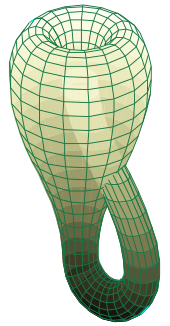
\includegraphics[width=6cm]{0_logo.png}
	\label{fig:logo}
\end{figure}

\vspace{2 cm}
\begin{center}
\Huge
\textbf{Seminar Topologie: Kompakte Räume}\\
\vspace{0.1 cm}
\Large
\textbf{Martin Kraus, Philipp Schwarz}
\vspace{1 cm}
\end{center}

\vfill

\end{titlepage}

%Inhaltsverzeichnis
\tableofcontents
%Abbildungsverzeichnis
\listoffigures
\addcontentsline{toc}{chapter}{Abbildungsverzeichnis}
%Tabellenverzeichnis
%\listoftabels
%\addcontentsline{toc}{chapter}{Tabellenverzeichnis}
\newpage

\pagenumbering{arabic}

% Die einzelnen Kapitel
\chapter{Vorwort}
Bevor wir beginnenn, möchten wir eine amüsante Anekdote, welche von Felix Bernstein übermittelt 
wurde, wieder geben. Diese ist ursprünglich in \cite{book:dedekind} S. 449 enthalten:

\begin{quote}
\glqq F. Bernstein übermittelt noch die folgenden Bemerkungen:
\glq \dots Von besonderem Interesse dürfte folgende Episode sein: Dedekind äußerte, hinsichtlich 
des Begriffes der Menge: er stelle sich eine Menge vor wie einen geschlossenen
Sack, der ganz bestimmte Dinge enthalte, die man aber nicht sähe, und von denen man
nichts wisse, außer daß sie vorhanden und bestimmt seien. Einige Zeit später gab Cantor
seine Vorstellung einer Menge zu erkennen: Er richtete seine kolossale Figur hoch auf,
beschrieb mit erhobenem Arm eine großartige Geste und sagte mit einem ins Unbestimmte 
gerichteten Blick: \glq Eine Menge stelle ich mir vor wie einen Abgrund.\grq \grq \grqq
\end{quote}

Auf die Frage, welche Überlegungen nun Cantor - den Schöpfer der Mengenlehre - 
zu solch einer Aussage bewogen hatten, kann sicherlich nur eine spekulative Antwort folgen.
Nichtsdestotrotz soll hier im Folgenden kurz ein Versuch gewagt werden. Ein Versuch der lediglich
eigener Anschauung entspringt und so logischer Strenge weder genügen kann noch will.

Man stelle sich, ausgehend von Dedekind, einen Sack vor der bestimmte Dinge enthält.
Dieser ist fest umrandet und somit gut greifbar für Verstand und Hand. Nun wird man
aber beobachten, dass beim Befüllen eines solchen Gebindes mit nur endlich vielen voluminösen Dingen 
die Kapazität des selbigen überschritten werden kann - das ewige \glqq Müllsackdilemma\grqq .
Was bei endlichen Mengen noch funktionieren kann, ist bei Undendlichen dann aber zum Scheitern verurteilt.

Da ist es doch gleich viel besser, einen Abgrund zur Hand zu haben, am Besten unendlich tief. So wäre
das Problem des Befüllens gelöst, jedoch sollte diese Vorstellung, der unendlichen Tiefe wegen, für unseren
Verstand nicht mehr all zu gut zugänglich sein.

Die vorliegende Seminararbeit befasst sich mit dem Begriff der kompakten Räume aus der mengentheoretischen
Topologie. Ein Begriff, der eine Brücke schlägt zwischen dem für uns greifbaren endlichen und dem
unendlichen - also dem Sack und dem Abgrund, wenn man so will.

Hauptziel dieser Seminararbeit ist es, den Satz von Heine-Borel zu beweisen. Also dass eine Teilmenge des
\(\mathbb{R}^n\) genau dann ein kompakter Unterraum ist, wenn sie beschränkt und abgeschlossen ist.
Des Weiteren werden einige Verallgemeinerungen von bereits aus der Analysis bekannten Sätzen abfallen.
Hier sei der Satz von Bolzano-Weiherstraß als Beispiel erwähnt.

Als Quellen für diese Ausarbeitung dienten vorallem die Bücher \cite{book:broeker} und \cite{book:jaenich}.
%
% - 1 kapitel allgemiene Definitonen (siehe kraus-schwarz)
% - 2 kapitel Komplakte Räume
%     - allgemeine eigenschaften (übergang zum Abgeschlsossenen)
%     - motivation
% - 3 Sätze zu Kompakten Räumen
%     - maximum / minimum (philipp)
%     - weiher straß (martin)
%     - Heine Borell
%


\chapter{Grundlegende Definitionen}

\begin{Def}[Topologischer Raum]
	Sei \(X\) eine Menge und \( \mathcal{O} \) eine Menge von Teilmengen von \(X\). Das Paar \((X,\mathcal{O})\) heißt topologischer Raum, wenn folgende Bedingungen erfüllt sind:
	\begin{enumerate}
		\item \( X, \emptyset \in \mathcal{O} \) 
		\item \( U_{i} \in \mathcal{O} \ \forall  i \in \{1, \dots, n\} 
			\Rightarrow \bigcap_{i=1}^n U_{i} \in  \mathcal{O} \)
		\item \( U_{\lambda} \in \mathcal{O} \ \forall \lambda \in \Lambda \Rightarrow \bigcup_{\lambda \in \Lambda} U_{\lambda} \)
	\end{enumerate}
\end{Def}
\textbf{Bemerkung:} Im Folgenden sei \((X,\mathcal{O})\) ein topologischer Raum.
\\
\textbf{Bemerkung:} Mengen \(O \in \mathcal{O} \) heißen offen. Eine Menge \(B \subset X\) heißt abgeschlossen, wenn ihr Komplement \( X \backslash A\) offen ist.

\begin{Def}[Umgebung eines Punktes] 
	Eine Menge \(U \subset X\) heißt \defH{Umgebung eines Punktes} \(p \in X\), wenn es eine offene Menge \(O \subset X\) gibt für die gilt: 
	\(p \in O \subset U\).
\end{Def}

\begin{Def}[Menge aller Umgebungen eines Punktes]
	Sei \(x \in X\) ein Punkt, dann bezeichnet \(U(x)\) die Menge aller Umgebungen von \(x\). 
\end{Def}

\begin{Def}[hausdorffsch]
	Ein topologischer Raum \((X,\mathcal{O})\) heißt \defH{hausdorffsch}, falls \( \forall x,y \in X\) mit \(x\ne y\) gilt:
	\[\exists U \in U(x) \mbox{ und } \exists V \in U(y) : U \cap V = \emptyset \]
\end{Def}

\begin{Def}[Offene Überdeckung]\label{def:ueberdeckung}
	Eine Familie \( (U_{\lambda} | \lambda \in \Lambda) \) mit \(U_{\lambda} \in \mathcal{O} \) für alle \( \lambda \in \Lambda \) heißt 	offene Überdeckung von X, wenn gilt:
	\[ \bigcup_{\lambda \in \Lambda } U_{\lambda} = X \]
\end{Def}
\textbf{Bemerkung:} Ist \(X \subset Y\) ein Teilraum und sind die \(U_{\lambda}\) offen in \(Y\), so heißt die Familie \( (U_{\lambda} | \lambda \in \Lambda) \) offene Überdeckung von
\(X\), wenn gilt \(X \subset \bigcup_{\lambda \in \Lambda} U_{\lambda}\).
\\
\textbf{Bemerkung:} \(\Lambda\) ist eine belibige Indexmenge. Ist diese endlicher Mächtigkeit, also \(|\Lambda| < \infty\), so nennt man auch die Überdeckung endlich. 
\\
\textbf{Bemerkung:} Eine Überdeckung \( (U_{\gamma} | \gamma \in \Gamma) \)  heißt Teilüberdeckung von \( (U_{\lambda} | \lambda \in \Lambda ) \), wenn \(\Gamma \subset \Lambda\). 

\begin{figure}[ht]%{0.50\columnwidth}
	\centering
	\def\svgwidth{150}
	\input{2_ueberdeckung.pdf_tex}
	\caption{Illustration zur Definition \ref{def:ueberdeckung}}
	\label{fig:ueberdeckung}
\end{figure}

\begin{Def}[Offene Kugel]
	Sei \((X,d)\) ein metrischer Raum, \(p \in X\) und \(\epsilon \in \mathbb{R}\). Dann nennt man
	\[ B_{\epsilon}(p) := \{ x \in X | d(p,x) < \epsilon \} \]
	offene Kugel um den Punkt \(p\) mit Radius \(\epsilon\) oder auch \(\epsilon-Umgebung\) von \(p\).
\end{Def}

\chapter{Kompakte Räume}
Im folgendenden Kapitel werden kompakte Räume definiert und motiviert. Weiterhin wird eine Charakterisierung jener Räume gegeben.
Nun aber endlich zur Definition von kompakten Räumen.

\begin{Def}[Kompaktheit]
	Ein hausdorffscher Raum \((X, \mathcal{O})\) heißt \defH{kompakt} wenn es zu jeder offenen Überdeckung 
	\((U_{\lambda} | \lambda \in \Lambda)\) von \(X\) eine endliche offene Teilüberdeckung gibt, wenn also gilt:
	\[ (U_{\lambda} | \lambda \in \Lambda) \mbox{ offene Überdeckung }
     \Rightarrow \exists \Gamma \subset \Lambda : |\Gamma| < \infty \land \bigcup_{\gamma \in \Gamma} U_{\gamma} = X \] 
\end{Def}
Man kann durch Übergang zu Komplementen folgende Charakterisierung finden:

\begin{Satz}[Charakterisierung Kompaktheit]
	Ein hausdorffscher Raum \((X, \mathcal{O})\) ist genau dann \textbf{kompakt}, wenn gilt:
	\begin{align*}
		(A_{\lambda}| \lambda \in \Lambda) \mbox{ Familie } & \mbox{in } X \mbox{ abgeschlossener Mengen mit } 
		\bigcap_{\lambda \in \Lambda} A_{\lambda} = \emptyset \\
		\Rightarrow \exists \Gamma \subset \Lambda : |\Gamma| < \infty & \land \bigcap_{\gamma \in \Gamma} A_{\gamma} = \emptyset
	\end{align*} 
\end{Satz}
\beweis{Beweis}
	\\
	\glqq\(\Leftarrow\)\grqq
	\\
	Gelte nun für beliebige Familien abgeschlossener Mengen \((A_{\lambda}| \lambda \in \Lambda)\) mit der Eigenschaft
	\(\bigcap_{\lambda \in \Lambda} A_{\lambda} = \emptyset\), dass eine endliche Teilmenge \(\Gamma \subset \Lambda\) existiert mit
	\(\bigcap_{\gamma \in \Gamma} A_{\gamma} = \emptyset\) und sei \( (U_{\omega} | \omega \in \Omega) \) offene Überdeckung
	von \(X\). So setze \(A_{\omega} = X \backslash U_{\omega} \; \forall \omega \in \Omega\), d.h. \(A_{\omega}\) ist abgeschlossen
	und es folgt 
	\[\bigcap_{\omega \in \Omega} A_{\omega} = \bigcap_{\omega \in \Omega} X \backslash U_{\omega} =  X \backslash 
	\bigcup_{\omega \in \Omega} U_{\omega} = X \backslash X =  \emptyset \]
	Nach Voraussetzung aber existiert ein endliches \(\Gamma \subset \Omega\), sodass die obige Gleichung erfüllt bleibt. Demnach ist 
	\[ X = X \backslash \emptyset = X \backslash \bigcap_{\gamma \in \Gamma} A_{\gamma} = \bigcup_{\gamma \in \Gamma} X \backslash A_{\gamma} = 
	\bigcup_{\gamma \in \Gamma} U_{\gamma} \] 
	und es ist zur Überdeckung \( (U_{\omega} | \omega \in \Omega) \) eine endliche Teilüberdeckung gefunden.
	\\
	\glqq\(\Rightarrow\)\grqq
	\\
	Die Hinrichtung zeigt man analog, indem man Kompaktheit voraussetzt und für eine Familie abgeschlossener Teilmengen zu den 
	offenen Komplementen übergeht.
\qed\\
%
\section{Beispiel}
Man betrachte die Menge \( (0,1) \subset \mathbb{R} \).\\ Auf den ersten Blick ist nicht klar, warum diese Menge, laut unserer Definition, nicht kompakt ist. 
Nehme man zum Beispiel die offene Überdeckung \( S_{n} := (-n,n) \subset \mathbb{R} , n \in \mathbb{N} \), diese überdeckt sogar ganz \(  \mathbb{R} \). 
Und \( S_{1} = (-1,1)  \) überdeckt schon unsere ganze Menge \( (0,1) \). \\
Also hat \( (S_{n} | n \in \mathbb{N} ) \) eine endliche offene Überdeckung die ganz \( (0,1)\) überdeckt.
Aber laut Definition von kompakten Räumen muss jede offene Überdeckung eine endliche offene Teilüberdeckung besitzen. Wir haben nun aber nur eine offene Überdeckung betrachtet. Betrachtet man nun nämlich die offene Überdeckung \( (U_{i}:= (0,1-\frac{1}{i})| i \in \mathbb{N}) \), so ist \(\bigcup_{i \in \mathbb{N}} U{i} = (0,1) \). Wenn \( (0,1)  \) kompakt wäre, 
so würde es nun eine Teilmenge \(I \subset \mathbb{N} \) geben mit \(\bigcup_{i \in I} = (0,1) \).
Da \(I\) eine endliche Teilmenge ist, besitzt \(I\) ein Maximum \( m \in \mathbb{N} \). Wählt man \(x \in (1-\frac{1}{m},1) \), dann ist \(x \in (0,1) \) aber nicht in 
\(\bigcup_{i \in I} U_{i}\). Also war die Annahme falsch, dass jede offene Überdeckung eine endliche Teilüberdeckung enthält. Daher ist die Menge \((0,1) \) nicht kompakt.\\
%		
\section{Motivation}
Warum ist denn Kompaktheit überhaupt eine beachtenswerte Eigenschaft? Nun, sie ist sozusagen ein Bindeglied zwischen dem 
Endlichen und dem Unendlichen - zwischen Säcken und Abgründen. Ein Kompakter Raum seinerseits 
kann durchaus unendlich, ja sogar überabzählbar unendlich viele Elemente enthalten. Überdecken kann man diese aber immer mit
einem endlichen System aus offenen Teilmengen des Raumes. Somit ist auf kompakten Räumen folgende Schlussweise möglich:
\\
\begin{Satz}
	Sei \( (X, \mathcal{O}) \) ein kompakter Raum, \(O \in \mathcal{O}\) und 
	\( \Psi(O) : \mbox{\glqq} O \mbox{ hat die Eigenschaft } \psi \mbox{\grqq} \) eine Aussage, 
	daher trifft die Eigenschaft \(\psi\) entweder auf \(O\) zu, oder eben nicht.
	Gilt nun weiter:
	\begin{align}
		U, V \in \mathcal{O} : \Psi(U) \land \Psi(V) &\Rightarrow \Psi(U \cup V) \label{eq:motivation:1}\\
		\forall x \in X \; \exists U_x \in \mathcal{O}, x \in U_x &: \Psi(U_x) \label{eq:motivation:2}
	\end{align}
	Dann ist auch \(\Psi(X)\) wahr, d.h. es gilt die Eigenschaft \(\psi\) für \(X\).
\end{Satz}
%
\beweis{Beweis}
	Es bildet \( (U_x | x \in X) \) wegen \eqref{eq:motivation:2} eine offene Überdeckung von \(X\). Aus der Kompaktheit von \(X\) folgt nun 
	die Existenz einer endlichen Teilüberdeckung, also \(X =  \bigcup_{i=1}^{n} U_{x_i}\) mit geeignetem \( n \in \mathbb{N} \). 
	Mittels vollständiger Induktion zeigt man, dass \(\Psi(X)\) wahr ist.
	\\
	\\
	\underline{Induktions Anfang}: \(\Psi(\bigcup_{i=1}^{1} U_{x_i}) = \Psi(U_{x_1}) \) ist wahr nach \eqref{eq:motivation:2}.
	\\
	\underline{Induktions Voraussetzung}: Sei nun \( \Psi(\bigcup_{i=1}^{k} U_{x_i}) \) erfüllt.
	\\
	\underline{Induktions Schritt}: Nach (I.V.) und \eqref{eq:motivation:2} ist \(\Psi(\bigcup_{i=1}^{k} U_{x_i}) \land \Psi(U_{x_{k+1}})\) wahr.
	Nun Folgt aus \eqref{eq:motivation:1}, dass \( \Psi(\bigcup_{i=1}^{k} U_{x_i} \cup U_{x_{k+1}}) = \Psi( \bigcup_{i=1}^{k+1} U_{x_i} ) \) erfüllt ist.
	\\
	\\
	Also ist \(\Psi(X) =  \Psi(\bigcup_{i=1}^{n} U_{x_i})\) wahr.
\qed
\\
\\
Man beachte, dass hier Vollständige Induktion nur anwendbar ist, da eine endliche offene Teilüberdeckung von \( (U_x | x \in X) \) existiert bzw. \(X\) kompakt ist.
Ist zum Beispiel die Funktion \(f : X \to \mathbb{R}\) lokal beschränkt, d.h. zu jedem \(x \in X\) existiert eine Umgebung \(U_x\), mit \(f(U_x)\) ist beschränkt, 
dann ist schon \(f\) beschränkt (Für \(U,V \in \mathcal{O}\) ist \(f(U \cup V)\) durch das Minimum der unteren und das Maximum der oberen 
Schranken von \(f(V), f(U)\) beschränkt). Setzt man \(f(x):=\frac{1}{x}\) und \(X:=(0,1)\), so ist \(f\) lokal beschränkt.
Für \(f(X)\) jedoch lässt sich keine obere Schranke angeben, weil \((0,1)\) nunmal nicht kompakt ist.



\chapter{Sätze über kompakte Räume}

\section{Satz von Heine-Borel}
%
Hier ist eine kleine Skizze, die deutlich machen soll, welche Sätze wir als Zutaten für unser Endprodukt, den \glqq Satz von Heine-Borel\grqq, brauchen. \\
%
\\
\input{heineborel_skizze0.pdf_tex}
%

\begin{Satz}\label{satz:beschr}
	Ein kompakter Teilraum \(K\) eines metrischen Raumes \( (X, d) \) ist beschränkt, daher es gilt:
	\[ \exists p \in K, n \in \mathbb{N} : K \subset B_n(p) := \{ x \in X | d(x,p) < n \} \]
\end{Satz}
\beweis{Beweis} 
	Sei \(p \in K\). Das System \( (B_{n}(p) | n \in \mathbb{N}) \) der offenen Kugeln um \(p\) vom Radius \(n \in \mathbb{N}\) 
	überdeckt den gesamten metrischen Raum \(X\), da man für jedes \(x \in X\) ein \(n \in \mathbb{N}\) findet mit \(d(p,x) < n\),
	also mit \(x \in B_{n}(p)\).
	So gilt \(K \subset X = \bigcup_{n \in \mathbb{N}} B_{n}(p)\) und es wird insbesondere auch \(K\) überdeckt. 
	Da \(K\) kompakt ist gibt es ein \(m \in \mathbb{N} : K \subset \bigcup_{i=1}^{m} B_{i}(p) \). Hier ist
	mit eingegangen, dass jede endliche Teilmenge von \(\mathbb{N}\) ein Maximum besitzt.
	Weiterhin gilt \( B_0(p) \subset B_1(p) \subset \dots \subset B_m(p) \) und es folgt \(K \subset B_m(p)\).
\qed

\begin{figure}[ht]
	\centering
	\def\svgwidth{200}
	\input{4_beschraenktheit.pdf_tex}
	\label{fig:beschraenktheit}
	\caption{Illustration zu Satz \ref{satz:beschr}}
\end{figure}

\begin{Satz}\label{satz:intervall}
	Sei \(I := [ a , b ] \subset \mathbb{R}\) ein Intervall mit \(a<b\) und \(a,b \in \mathbb{R}\). Dann 
	ist \(I\) kompakt.
\end{Satz}
\beweis{Beweis} 
	Sei \( (U_{\lambda} | \lambda \in \Lambda) \) offene Überdeckung von \(I\). Zunächst zeigen wir,
	dass ein \(\delta > 0\) existiert mit der Eigenschaft: Für alle \(p \in I\) liegt \(B_{\delta}(p)\)
	in einem \(U_{\lambda}, \lambda \in \Lambda\). Dies kann man auch so ausdrücken: 
	\[ \exists \delta > 0 : \forall p \in I \mbox{ gilt } B_{\delta}(p) \subset U_{\lambda} \mbox { für ein } \lambda \in \Lambda \]
	Wir nehmen an, das Gegenteil sei der Fall:
	\[ \forall \delta > 0 : \exists p(\delta) \in I \mbox{ mit } B_{\delta}(p(\delta)) \not\subset U_{\lambda} \mbox { für alle } \lambda \in \Lambda \]
	Da diese Aussage für alle \(\delta > 0\) gilt, ist es erlaubt \(\delta = \frac{1}{n}\) zu setzen, wobei \(n \in \mathbb{N}\) ist.
	Somit haben wir auf dem Intervall \(I\) eine Folge \(p_{n} := p(\frac{1}{n})\) gefunden mit der Eigenschaft, dass für alle \(\lambda \in \Lambda\)
	gilt: \(B_{\frac{1}{n}}(p_{n}) \not\subset U_{\lambda}\). Nach dem aus der Analysis bekannten Satz von Bolzano-Weiherstraß gibt
	es zu jeder Folge auf dem Intervall \(I\) eine konvergente Teilfolge. Also dürfen wir zu einer konvergenten Teilfolge mit Limes \(p \in I\) übergehen.
  Konvergenz sagt ja gerade aus, dass es zu jeder Umgebung \(U\) von \(p\) ein \(n_0 \in \mathbb{N}\) gibt, 
	ab dem die Folgenglieder in dieser Umgebung verweilen. Dies wiederum heißt, es existiert ein \(B_{\epsilon}(p) \subset U_{\lambda}\) für ein \(\lambda \in \Lambda\)
	(\(p\) muss ja auch in irgendeinem Teil der Überdeckung liegen). Wählt man nun \(n\) so groß, dass \(p_n \in B_{\frac{\epsilon}{2}}(p)\) und \(\frac{1}{n} < \frac{\epsilon}{2}\),
	dann gilt:
	\[ x \in B_{\frac{1}{n}}(p_n) \Rightarrow |x-p| < |p-p_n+p_n-x| < |p-p_n| + |p_n-x| < \frac{\epsilon}{2} + \frac{1}{n} < \epsilon \Rightarrow x \in B_{\epsilon}(p) \]
	Damit ist \(B_{\frac{1}{n}}(p_n) \subset B_{\epsilon}(p) \subset U_{\lambda}\).
	Widerspruch zur Annahme und es gibt für alle \(p \in I\) ein \(\delta > 0\) mit \(B_{\delta}(p) \subset U_{\lambda}, \lambda \in \Lambda\).
	Zerlegt man \(I\) in endlich viele Teilintervalle mit Länge kleiner \(\delta\), so ist jeder dieser Abschnitte ganz in einem \(U_{\lambda}, \lambda \in \Lambda\)
	enthalten. Daher bilden eben jene \(U_{\lambda}\) eine endliche Überdeckung von \(I\).
\qed

\begin{Satz}\label{satz:abgeschlkomp}
		Ist \(X\) kompakt und \(A \subset X \mbox{ abgeschlossen } \Rightarrow A\) kompakt.
\end{Satz}
%
\beweis{Beweis} 
	\\
 	Sei \((F_{\lambda} | \lambda \in \Lambda) \) eine Familie abgeschlossener Teilmengen in \(A\) mit \( \bigcap_{\lambda \in \Lambda } F_{\lambda} = \emptyset \).\\
	Dann ist automatisch auch jedes \(F_{\lambda} \) abgeschlossen in \(X\).\\
	Da \(X\) kompakt ist, besitzt jede Familie \((B_{\omega} | \omega \in \Omega) \) in \(X\) abgeschlossener Mengen mit der Eigenschaft 
	\( \bigcap_{\omega \in \Omega} B_{\omega} = \emptyset\), eine 
	endliche Indexmenge \(\Phi \) für die bereits gilt: \( \bigcap_{\omega \in \Phi} B_{\omega} = \emptyset\).\\
	Also existiert auch eine endliche Indexmenge \( \Gamma \subset \Lambda \) mit \( \bigcap_{\lambda \in \Gamma } F_{\lambda} = \emptyset \), dadurch ist 
	\(A\) auch kompakt.
\qed
		
\begin{Satz}\label{satz:kompabgeschl}
	Ist \(X\) hausdorffsch und \(A \subset X \) kompakt \( \Rightarrow \) \(A\) ist abgeschlossen.
\end{Satz}
%
\beweis{Beweis}
	\\
	Wir wollen zeigen, dass es für jeden Punkt in \(X \backslash A \) eine offene Umgebung in \(X \backslash A \) gibt. Sei daher \(p \notin A \).
	Da \(X\) hausdorffsch ist gilt folgende Aussage:
	\[ \forall a \in A : \exists U_{a} \subset \mathcal{O} \mbox{ mit }  a \in U_{a} \mbox{ und } \exists V_{a}\subset \mathcal{O}, p \in V_{a} 
		 \mbox{ für die gilt } U_{a} \cap V_{a} = \emptyset \] 
	Weiterhin folgt aus der Kompaktheit von \(A\) die Existenz einer endliche Menge \(I \subset A\) mit der Eigenschaft:
	\[ \bigcup_{a \in I} U_{a} \supset A \]
	Nach Definition eines topologischen Raumes ist der endliche Schnitt \(\bigcap_{a \in I} V_{a}\) offen. Zusätzlich gilt 
	\(p \in \bigcap_{a \in I} V_{a} \subset  X\backslash A \), weil für jedes \(i \in I\) der Schnitt \( ( \bigcap_{a \in I} V_a ) \cap U_i = \emptyset \) ist und 
	somit dieser nicht in \(A\) liegt.
	Also ist eine offene Umgebung von \(p\) in \(X\backslash A\) gefunden und da \(p\) beliebig gewählt war, gilt dies für 
	jeden Punkt \(p \in X\backslash A\). Damit ist \(A\) abgeschlossen. 
\qed
	
\begin{Lemma}[Tubenlemma]\label{satz:tubenlemma}
	Sei \(K \) ein kompakter topologischer Raum,  \(p \in X \) und \( U \subset X \times K \) offen mit \( \{p\} \times K \subset U \). \\
	Dann \( \exists \; V \subset X \), \( V \in \mathcal{O} \) mit \( V \times K \subset U \). \( V \times K \) nennt man \textbf{Tubenumgebung} von 
	\( \{p\} \times K \subset X \times K \).
\end{Lemma} 
%
\beweis{Beweis}
	\\
	\( \forall k \in K \; \exists V_{k}, W_{k}\) offene Mengen mit \( p \in V_{k} \subset X, k \in W_{k} \subset K, (p,k) \in  V_{k} \times W_{k} \subset U\).
	Diese offenen Mengen \(V_{k}, W_{k}\) kann man finden, da laut Vorraussetzung \(U  \subset X \times K \) offen in der Produkttopologie ist.
	Da \(K \) kompakt ist, existiert eine endliche Teilmenge
	\( I \subset K \) mit \( \bigcup_{ k \in I } W_{k} = K \). Wähle \(V := \bigcap_{ k \in I } V_{k} \), dann gilt:
	\[ V \times K \subset \bigcup_{k \in I} (V_{k} \times W_{k}) \subset U \] \qed \newpage	
%
\begin{figure}[ht]
	\centering
	\def\svgwidth{200}
	\input{tubenlemma.pdf_tex}
	\label{fig:tubenlemma}
	\caption{Illustration zu Lemma \ref{satz:tubenlemma}}
\end{figure}\\
%
\begin{Satz}
	Ein endliches Produkt hausdorffscher Räume ist wieder hausdorffsch.
\end{Satz}
%
\beweis{Beweis}
	\\
	Wir wollen zunächst zeigen, dass das Produkt zweier hausdorffscher Räume wieder hausdorffsch ist. Dies reicht aus, da man jedes endliche Produkt topologischer Räume
	induktiv auf ein Produkt zweier Räume zurückführen kann. \\
	Seien \(X, Y\) zwei hausdorffsche topologische Räume.\\
	Seien weiter \( (p,q), (x,y) \in X \times Y \mbox{ wobei } (p,q) \ne (x,y) \). \\
	Laut Vorraussetzungen ist \(X\) und \(Y\) jeweils hausdorffsch, also folgt: 
	\begin{align}
		x &\ne p \mbox{ oder }\label{eq:produkt1}\\ 
		y &\ne q\label{eq:produkt2} 
	\end{align}
	Zu \eqref{eq:produkt1} da \(x \ne p \) ist, haben \(x, p \) Umgebungen \(A, B \) mit \( A \in U(x)  \land B \in U(p) \), für die gilt: \(A \cap B = \emptyset \).\\ Daher gibt es die
	zwei Umgebungen \( (A \times Y), (B \times Y) \) mit \( (A \times Y) \cap (B \times Y) = \emptyset \). \\
	Setzt man bei \eqref{eq:produkt2} mit dem gleichen Ansatz an, so folgt leicht, dass \( (X \times Y) \) hausdorffsch ist, da wir gerade gezeigt haben, falls mindestens eine Komponente
	nicht gleich ist, existieren fremde Umgebungen zu zwei nicht gleichen Punktepaaren\( (p,q), (x,y) \), was genau der Definition von hausdorffsch entspricht.
\qed

\begin{Satz}\label{satz:prodkomp}
	Ein endliches Produkt kompakter Räume ist wieder kompakt.
\end{Satz}
	%
	\beweis{Beweis}
	\\
	Wir zeigen wieder zunächst, dass das Produkt zweier kompakter Räume wieder kompakt ist. Hier kann man ebenfalls leicht mittels Induktion jedes endliche Produkt kompakter Räume 
	auf ein Produkt zweier kompakter Räume zurückführen. \\
	Nun seien \(X, Y\) zwei kompakte Räume.\\
	Ist \((U_{\lambda} | \lambda \in \Lambda) \) eine offene Überdeckung in \(X \times Y \). Jede Faser \( \{p\} \times Y, p \in X \) wird von endlich vielen \(U_{\lambda} \) überdeckt,
	da Y kompakt ist. Also gibt es eine Teilmenge \( I \subset \Lambda \) mit \( \{p\} \times Y \subset \bigcup_{ \lambda \in I } \{p\} \times U_{\lambda} \). 
	Nach dem Tubenlemma überdeckt \( \bigcup_{ \lambda \in I } \{p\} \times U_{\lambda} \) noch eine Menge \(\bigcup_{ p \in X } V_{p} \times Y \mbox{ mit } V_{p} \in X \),
	 wobei \( V_{p} \) eine offene Umgebung von \( p \in X \) ist. Da X kompakt ist überdecken, auch hier bereits endlich viele \(V_{p} \mbox{ ganz } X \). 
\qed

\begin{figure}[ht]
	\centering
	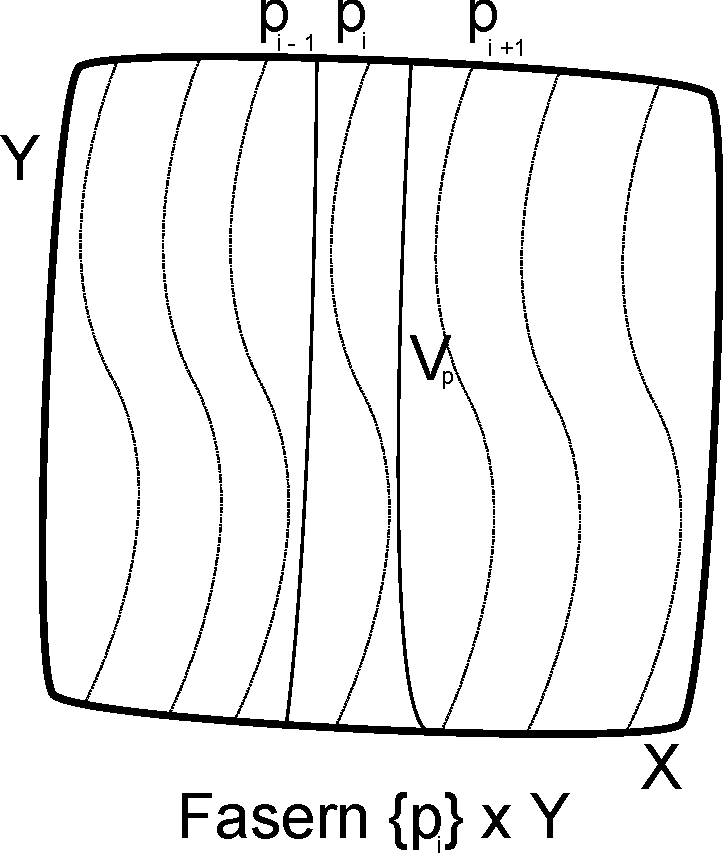
\includegraphics[width=6cm]{produkt_kompakter_raueme.pdf}
	\label{fig:satzprodkomp}
	\caption{Illustration zu Satz \ref{satz:prodkomp}}
\end{figure}
	
\textbf{Bemerkung:} Der Satz von Tychoff zeigt sogar, dass überabzählbare Produkte kompakter Räume wieder kompakt sind. \\
%
\\
Nun können wir endlich zu unserem Hauptziel nämlich dem Satz von Heine-Borel zurück kommen.
%	
\begin{Satz}[Heine-Borel]
	Eine Teilmenge  \( A \subset \mathbb{R}^n \) ist kompakt \(\Leftrightarrow A \) ist abgeschlossen und beschränkt.
\end{Satz}
%
\beweis{Beweis} \\
	Zu \(\Leftarrow \): \\
	Jede abgeschlossene und beschränkte Menge \(A \subset\mathbb{R}^n \), liegt in einem abgeschlossenen n-dimensionalen Würfel
	\( Q_r:= \{ x \in \mathbb{R}^n | \; |x_i| \leq r \quad i=1, \dots, n\} \subset \mathbb{R}^n \). 
	Dies folgt sofort aus der Beschränktheit der Menge \(A\). Der Würfel \(Q_r\) ist als Produkt abgeschlossener und beschränkter Intervalle nach den Sätzen \ref{satz:prodkomp} und \ref{satz:intervall} kompakt.
	Mit Satz \ref{satz:abgeschlkomp} folgt die Kompaktheit der darin enthaltenen abgeschlossenen Mengen.
	\\
	Zu \(\Rightarrow \): \\
	Sei \( K \subset \mathbb{R}^n \) kompakt, dann ist sie laut Satz \ref{satz:kompabgeschl} abgeschlossen und wegen Satz \ref{satz:beschr} ist sie auch beschränkt.
\qed \\
%
\\
\textbf{Bemerkung:} Wichtig ist hierfür aber die Vorraussetzung, dass der topologische Raum, der \(\mathbb{R}^n \) ist. Für metrische Räume ist dieser Satz nicht allgemein gültig. 
Da zum Beispiel mit der trivialen Metrik jede Menge beschränkt ist.
\\
%
Dieser enorm wichtige Satz hat die wunderbare Eigenschaft, dass man in einem sehr oft angewandten Raum, nämlich dem \(\mathbb{R}^n \), 
jetzt relativ leicht entscheiden kann ob eine Teilmenge kompakt ist. 

\section{Weitere}
% 
\begin{Satz}\label{satz:ftk:kompakt}
	Sei \( (X, \mathcal{O}_x) \) ein kompakter Raum und \((Y, \mathcal{O}_y)\) hausdorffscher Raum, sowie \\
	\(f: X \to Y\) stetig.
	Dann ist auch das Bild \( f(X) \) kompakt.
\end{Satz}
%
\beweis{Beweis}
	\\
	Sei \( (U_{\lambda} | \lambda \in \Lambda) \) eine offene Überdeckung von \(f(X)\). Es ist zu zeigen,
	dass eine endliche Teilüberdeckung existiert. 
	\[ f(X) = \bigcup_{\lambda \in \Lambda} U_{\lambda} \Rightarrow X = 
  	 f^{-1}(\bigcup_{\lambda \in \Lambda} U_{\lambda}) = 
		 \bigcup_{\lambda \in \Lambda} f^{-1}(U_{\lambda}) \]
	Da \(f\) stetig ist, sind die Urbilder \( f^{-1}(U_{\lambda}) \) der offenen Mengen \(U_{\lambda}\) wieder offen für 
	alle \(\lambda \in \Lambda\). Somit ist \( ( f^{-1}(U_{\lambda}) | \lambda \in \Lambda ) \) eine offene Überdeckung
	von \(X\). Zu dieser gibt es aufgrund der Kompaktheit von \(X\) ein endliches \( \Gamma \subset \Lambda \), mit 
	der Eigenschaft \( X = \bigcup_{\gamma \in \Gamma} f^{-1}(U_{\gamma}) \). Hieraus folgt:
	\[ f(X) = f(\bigcup_{\gamma \in \Gamma} f^{-1}(U_{\gamma})) = 
  	 \bigcup_{\gamma \in \Gamma} f(f^{-1}(U_{\gamma})) = 
	   \bigcup_{\gamma \in \Gamma} U_{\gamma} \]
\qed

\begin{Satz}
	Sei \((X, \mathcal{O})\) ein kompakter Raum. Dann ist eine stetige Funktion \(f: X \mapsto \mathbb{R}\) 
	beschränkt und nimmt ein Minimum und Maximum an.
\end{Satz}
%
\beweis{Beweis}
	Nach Satz \ref{satz:ftk:kompakt} ist das Bild von \( f(X) \subset \mathbb{R} \) kompakt. Mit Heine-Borel 
	folgt sofort die Beschränkt- und Abgeschlossenheit. Daher enthält \(f(X)\) sein Supremum und Infimum.
\qed
	\begin{Satz}[Satz von Bolzano-Weierstraß]
		Jede Folge in einem kompakten metrischen Raum \(K\) besitzt eine konvergente Teilfolge.
	\end{Satz}
	%
	\beweis{Beweis}\\
		Wir betrachten für beliebige \( p \in K \), die offenen Kugeln \( B_{\frac{1}{n}}(p) \) um \(p \), mit dem Radius \( \frac{1}{n},\; n \in \mathbb{N}\). \\
		Wir nehmen nun an, die Folge besitzt keine konvergente Teilfolge, also in jeder offenen Kugel \( B_{\frac{1}{n}}(p) \) findet man nur endlich viele Folgenglieder. 
		Da K kompakt ist, überdecken endlich viele  \( B_{\frac{1}{n}}(p) \) den ganzen Raum \( K \), daher hätte die Folge insgesamt nur endlich viele Folgenglieder.\\
		Das ist aber ein Widerspruch, da die ganze Folge mit unendlich vielen Folgengliedern im Raum \(K \) wohnt. Also war die Annahme falsch und somit besitzt jede Folge in einem kompakten
		Raum eine konvergente Teilfolge.
	\qed\\
	%
	{\bf Bemerkung:} Die Aussage dieses Satzes ist natürlich äquivalent mit der Aussage, das jede Folge in einem kompakten Raum mindestens einen Häufungspunkt besitzt. 
	%
	


% Anhang (Screenies etc.)
%\textcolor{white}{\cite{book:jaenich}\cite{book:broeker}}
\include{x_anhang}

\renewcommand{\bibname}{Quellenverzeichnis}
\bibliographystyle{geralpha}
\bibliography{document}

\end{document}

